In this chapter we will investegate the effect of the Boussinesq approximation on the plasma.

\section{Steady state profiles}
Starting with the profiles
%
\begin{figure}[htb]
    \centering
    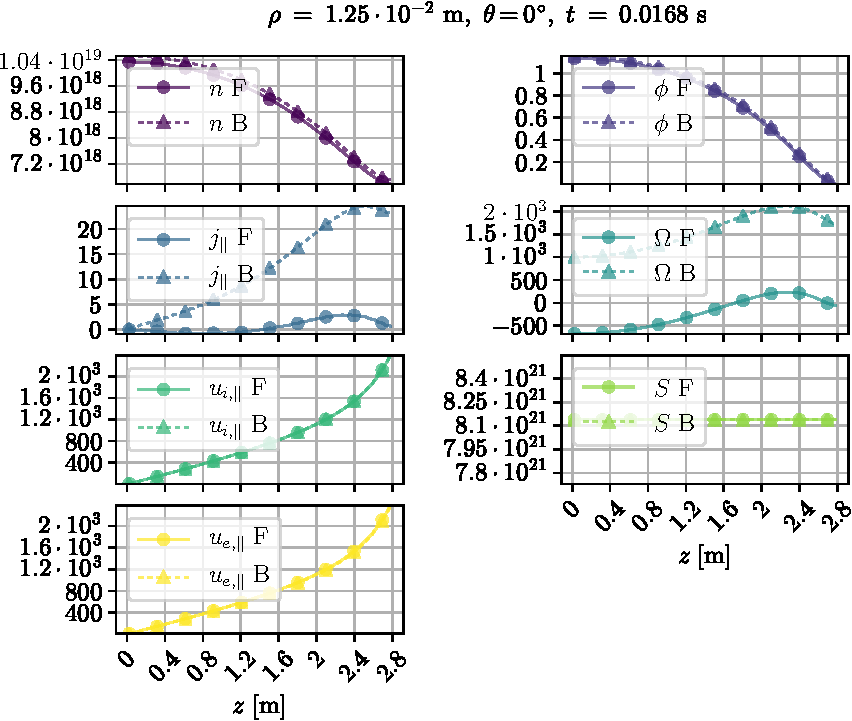
\includegraphics[width=1.0\textwidth]{fig/results/compareBouss/1DProfRad001B}
    \caption{Radial steady state profiles with and without the Boussinesq approximation.}
    \label{fig:compareBoussProfRad}
\end{figure}
%
We note that any difference between the model using the Boussinesq approximation and the one which do not lays in the vorticity equation.
Both terms affecting the background profile and terms affecting the fluctuations are affected.
Knowing this, there is no surprise that the vorticity profile has changed.
This in turn changes the perpendicular potential profile%
%
\footnote{One could say that it is the potential which determines the vorticity through $\Om = \grad_perp^2 \phi$, but since we are evolving the vorticity in time we are instead inverting the equation for $\phi$.
In that respect $\Om$ determines $\phi$.}%
%
.
Finally the parallel current profile is also sligthly changed.
This comes from that the balancing terms in the vorticity equation has changed.
The $\ve{E}\times\ve{B}$ advection terms are not active during the steady state as $\phi$ is axisymmetric.
However, the source term directly affects the profiles as seen in equation ...
also, the density plays a different role as explained in ...
%
\begin{figure}[htb]
    \centering
    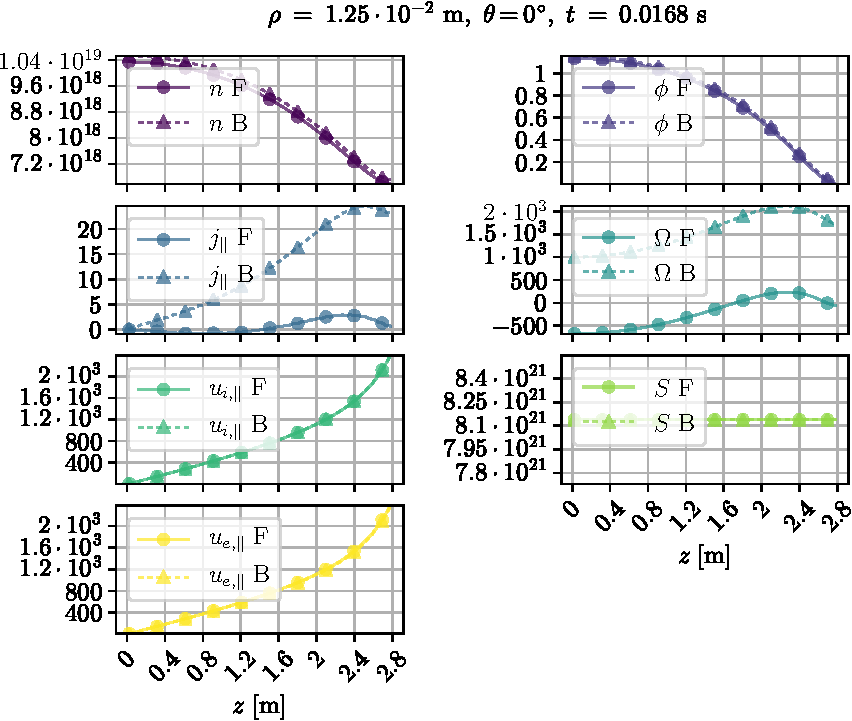
\includegraphics[width=1.0\textwidth]{fig/results/compareBouss/1DProfPar001B}
    \caption{Parallel steady state profiles with and without the Boussinesq approximation.}
    \label{fig:compareBoussProfPar}
\end{figure}
%
In the parallel direction, the changes are less pronounced.
To a high degree, the system follows a Boltzmann distribution.
Although the parallel ion velocity and the parallel electron velocity are almost the same as in the non-Boussinesq case, the small difference can clearly be seen in the parallel current.
In the Boussinesq case, this is much higher.
Again this comes from the change in the balancing terms in the vorticity equation.
Although the oscillating patterns in the parallel current is still there, they are much less pronounced due to the higher values of $j_\|$.
%


\section{The linear state}
%
The $\ve{E}\times\ve{B}$ advective terms plays a large role in the linear phase, as in particular these terms provides a way to couple modes by that make the energy and enstrophy cascade.
This is examplified in \cref{fig:compFFTB}.
%
\begin{figure}[htbp]
    \centering
    \begin{subfigure}[h]{0.45\textwidth}
        \centering
        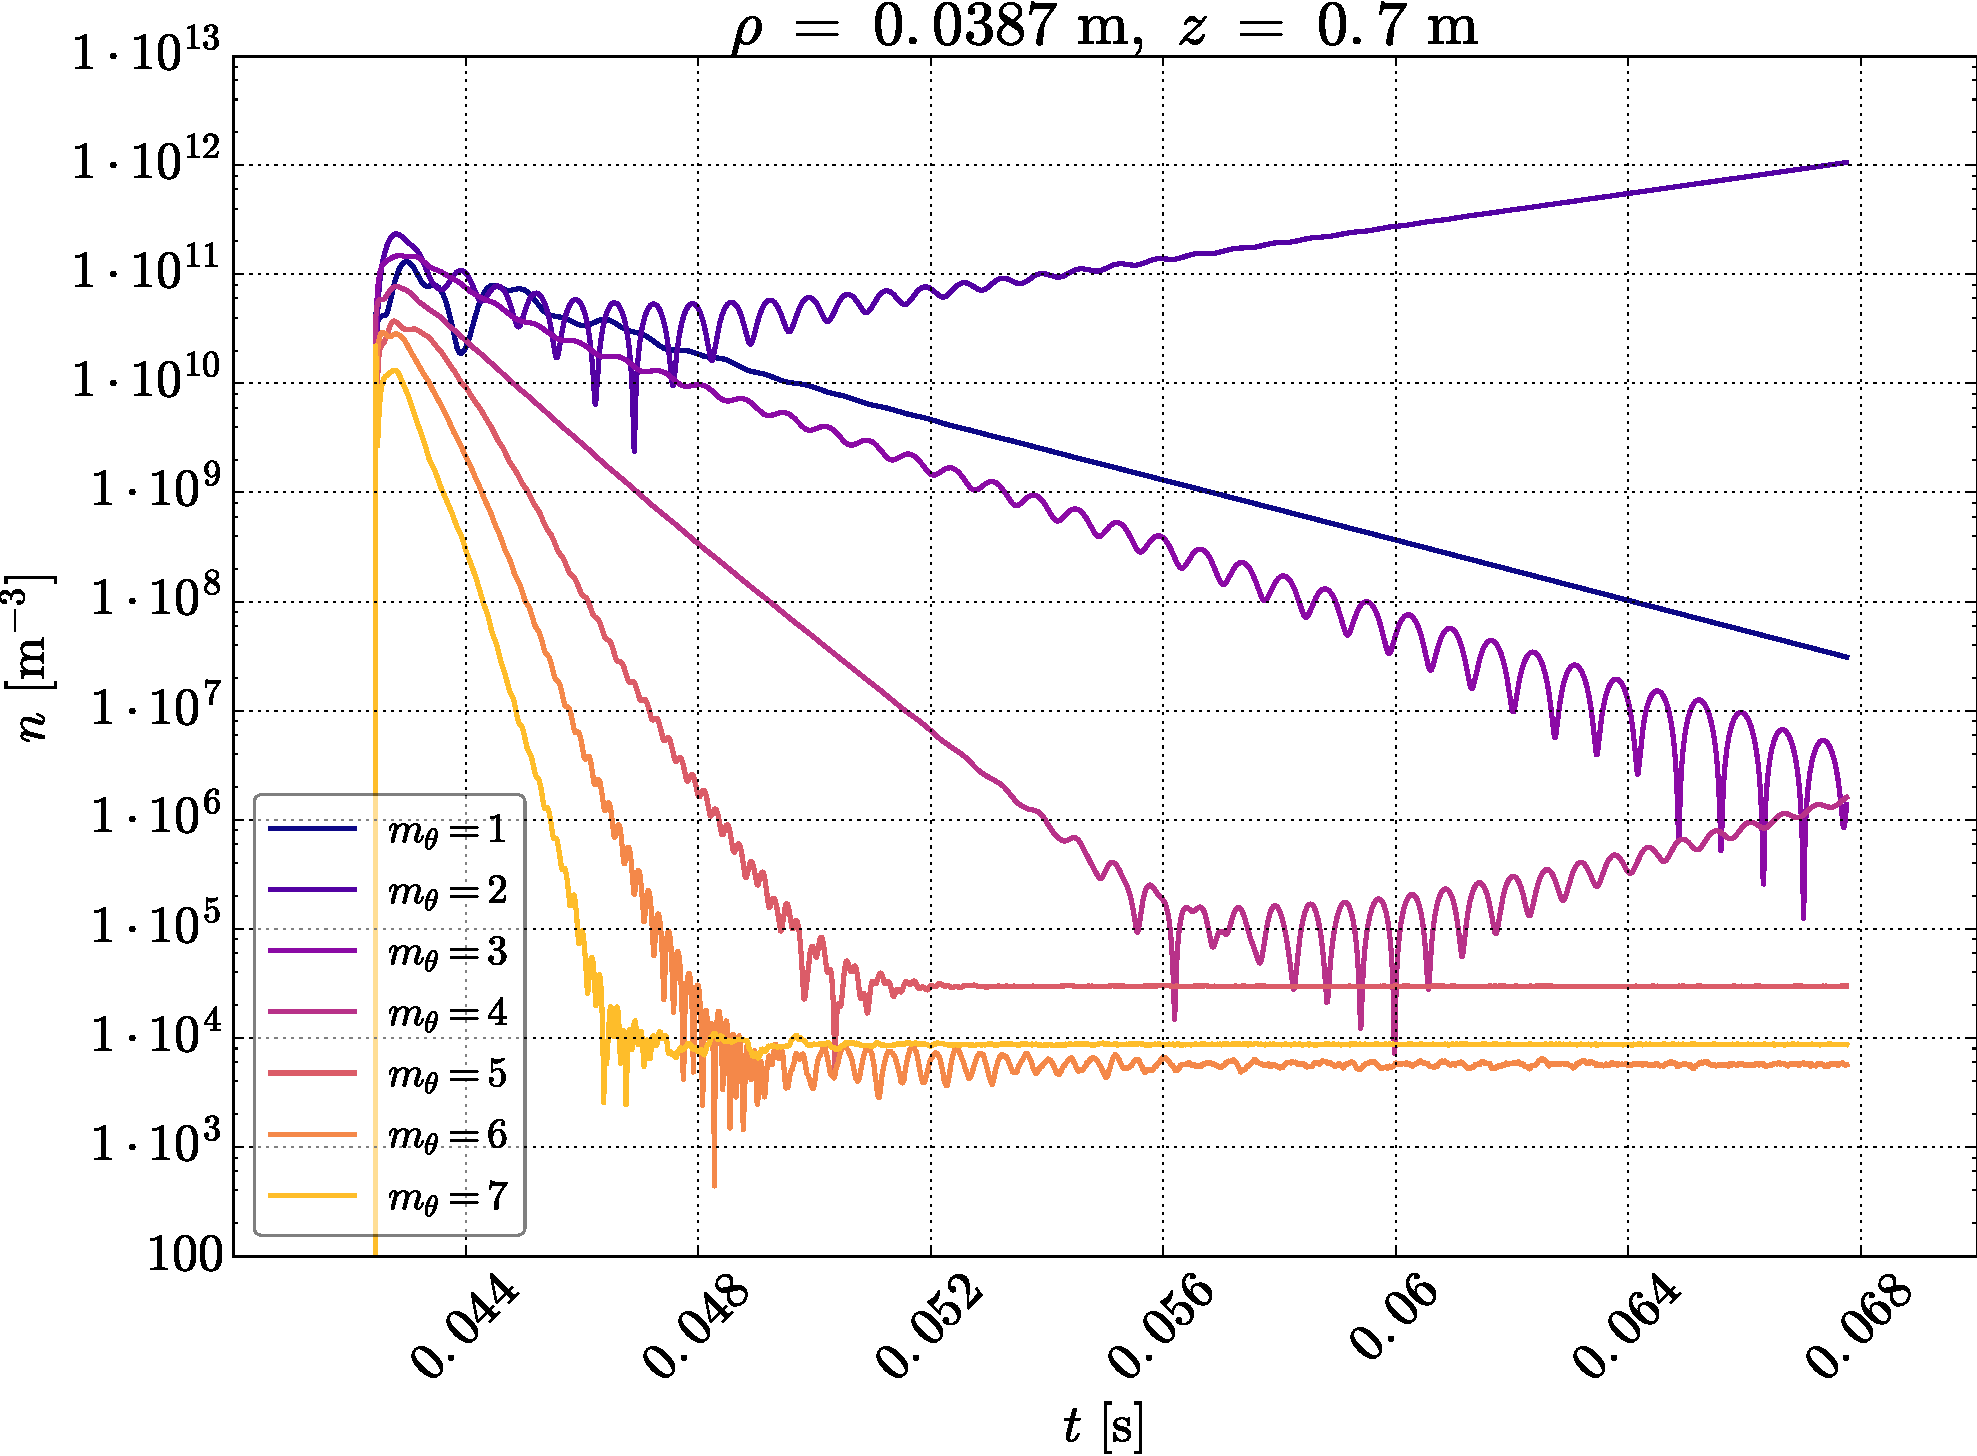
\includegraphics[width=1.0\textwidth]{fig/results/compareBouss/FFT004}
        \caption{Without the Boussinesq approximation}
        \label{fig:FFTWOB}
    \end{subfigure}%
    \hfill
    \begin{subfigure}[h]{0.45\textwidth}
        \centering
        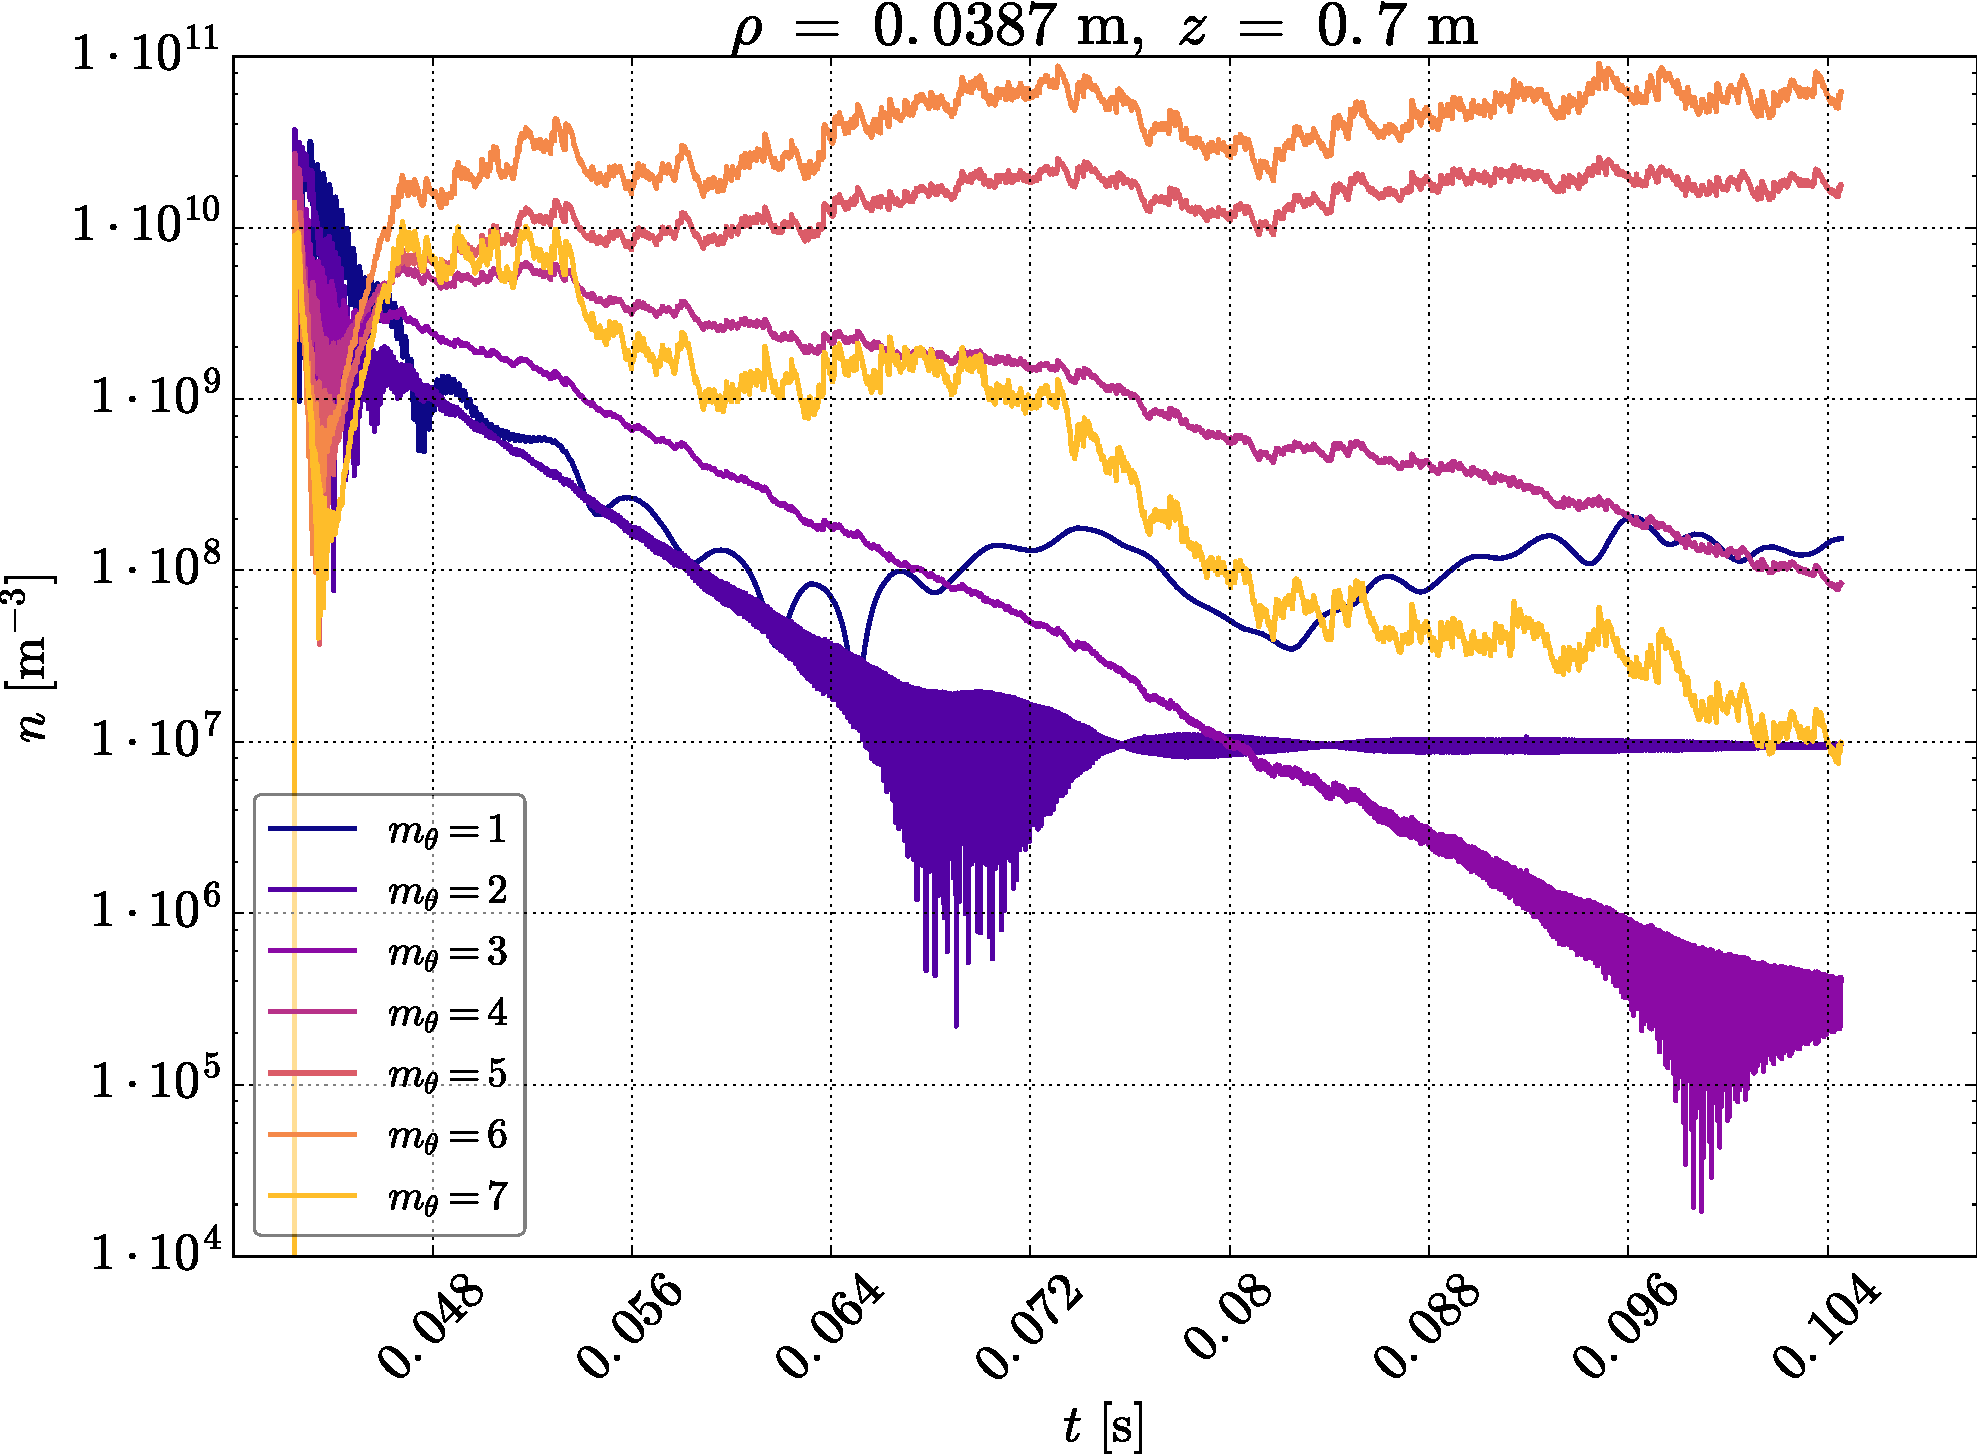
\includegraphics[width=1.0\textwidth]{fig/results/compareBouss/FFT004B}
        \caption{With the Boussinesq approximation.}
        \label{fig:FFTWB}
    \end{subfigure}
    \caption{Fourier modes of the density at $B=0.04\T$}
    \label{fig:compFFTB}
\end{figure}
%
While the \nth{2} mode grows in the non-Boussinesq case, no mode seems to be exponential growing when using the Boussinesq approximation.
%
\begin{figure}[htbp]
    \centering
    \begin{subfigure}[h]{1.00\textwidth}
        \centering
        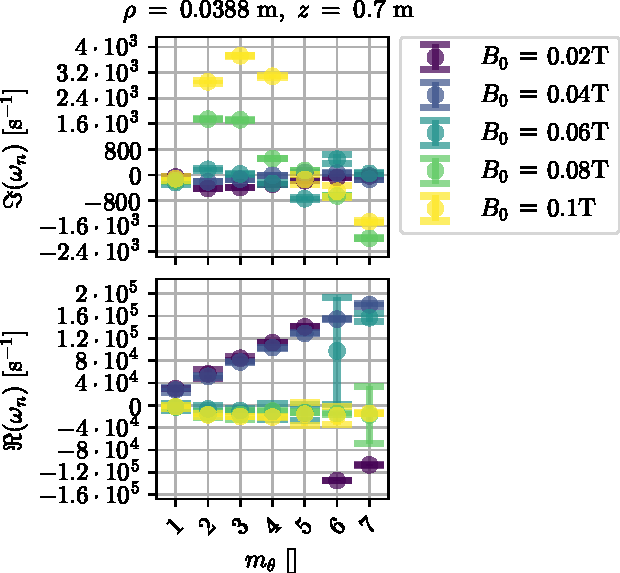
\includegraphics[width=1.0\textwidth]{fig/results/compareBouss/growthRatesB0Bous}
        \label{fig:grBBous}
    \end{subfigure}%
    \\
    \begin{subfigure}[h]{1.00\textwidth}
        \centering
        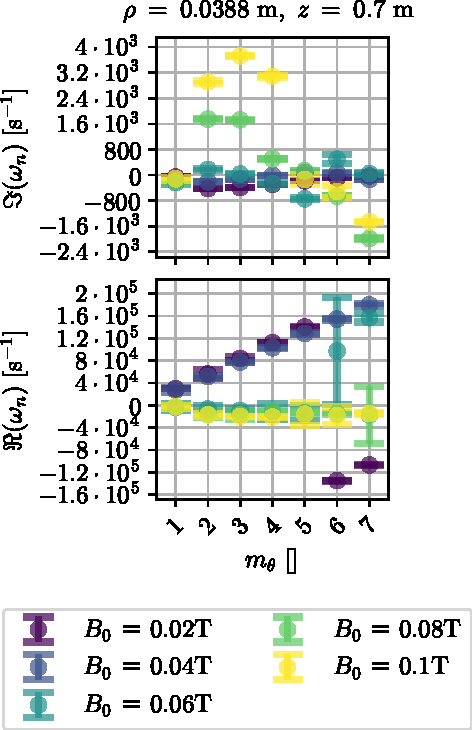
\includegraphics[width=1.0\textwidth]{fig/results/compareBouss/growthRatesB0ModeNr}
        \label{fig:grBModeNrBous}
    \end{subfigure}
    \caption{$B$-dependency on growth rates when using the Boussinesq approximation.}
\end{figure}
%
The difference in the linear growth rates can be furhter examined by comparing \cref{fig:grBBous, fig:grBModeNrBous} to
we see that the most unstable mode occurs for a lower mode number when using the Boussinesq approximation.
In absolute value the growth rates are around half as steep, and the rotation of the modes are larger with almost an order of magnitude when using the Boussinesq approximation.


\section{The turbulence phase}
%
There is also a large differences between the Boussinesq and the non-Boussinesq case in the turbulent state.
When investegating the energy in \cref{fig:energies008B} we notice three things.
%
\begin{figure}[htb]
    \centering
    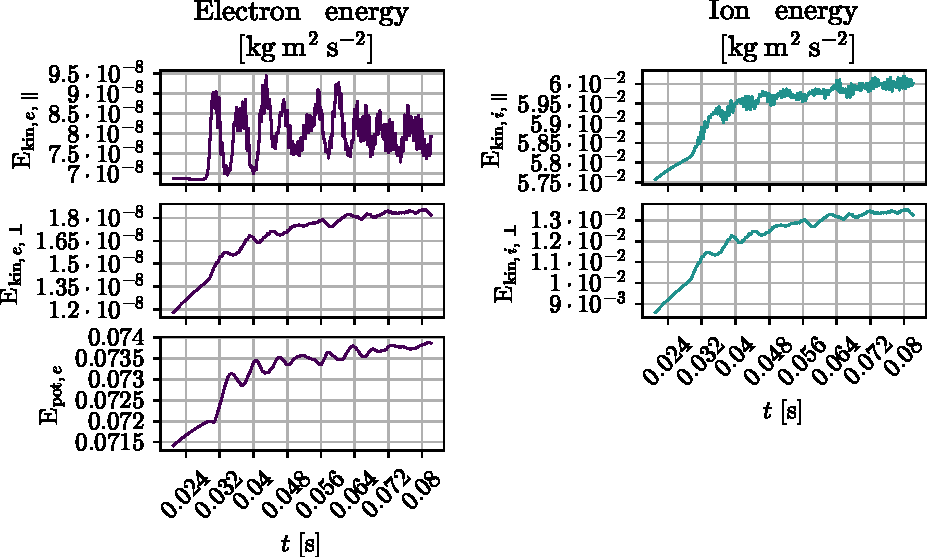
\includegraphics[width=1.0\textwidth]{fig/results/compareBouss/energies008B}
    \caption{Time trace of the energy for $B=0.08\T$ using the Boussinesq approximation.}
    \label{fig:energies008B}
\end{figure}
%
Firstly, in contrast to what is observed in simulations without the Boussinesq approximation, the energy is increasing in the linear phase (with exception of the paralell electron energy, which after close inspection actually shows a sligth decrease in the linear phase).
For the potential energy, this means that the total number of particles in the system is increasing as the electron temperature is constant.
If the density is increasing, this would also explain why the other energies are increasing as well.
The parallel electron energy can then only be decreasing if the parallel electron velocity is decreasing.

Next, we do not observe the energy overshoot as we did when investegating the simulations without the Boussinesq approximation.
This can also be seen by visual inspection the temporal evolution of the fields.
The dynamics does not appear to be faster during the onset of the turbulence then during the turbulent state.

Finally, the energy appears to be drifting to higher values with time.
In absolute terms, the energy is also larger when using the Boussinesq approximation.

This can also be seen if when investegating the temporal evolution of the fields.

Visual inspection of the fields also shows that the eddies evolve slower in the turbulence phase as when compared to the non-Boussinesq case, and it appear to be rotating clockwise.
This is shown in

INSERT T MAYBE 5 TRACES.

\section{Fluctuations}
%
The rotation of the plasma structure is also apparent in the time traces of $n$ in the three positions around the maximum gradient.
This is shown in \cref{fig:comb008B}.
%
\begin{figure}[htb]
    \centering
    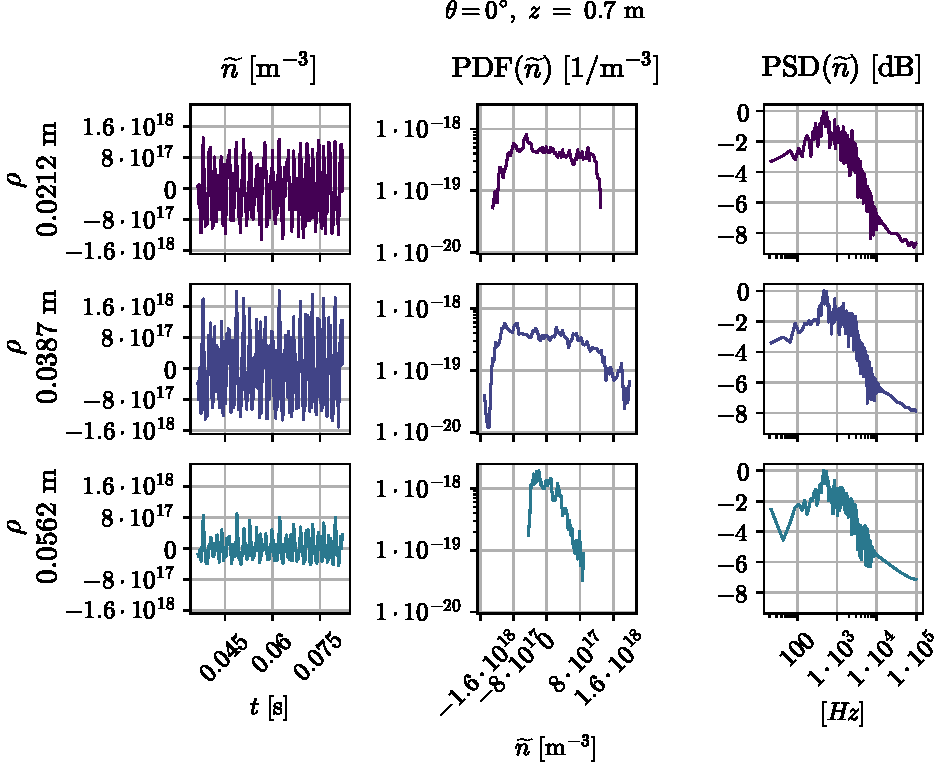
\includegraphics[width=1.0\textwidth]{fig/results/compareBouss/comb008B}
    \caption{Time traces in three fixed positions around the maximum gradient.}
    \label{fig:comb008B}
\end{figure}
%
The fluctuation spectrum is narrower and peaks at a frequency appromimately $3$ time as high as compared with the non-Boussinesq case.

The system using the Boussinesq approximation experience less flattening of the profiles as indicate in \cref{}.
Outside the position of the absolute maximum gradient the density profile follows the steady state profile to a good degree.
Furthermore, the potential is shifter closer to the absolute maximum of the gradient.
%
\begin{figure}[htb]
    \centering
    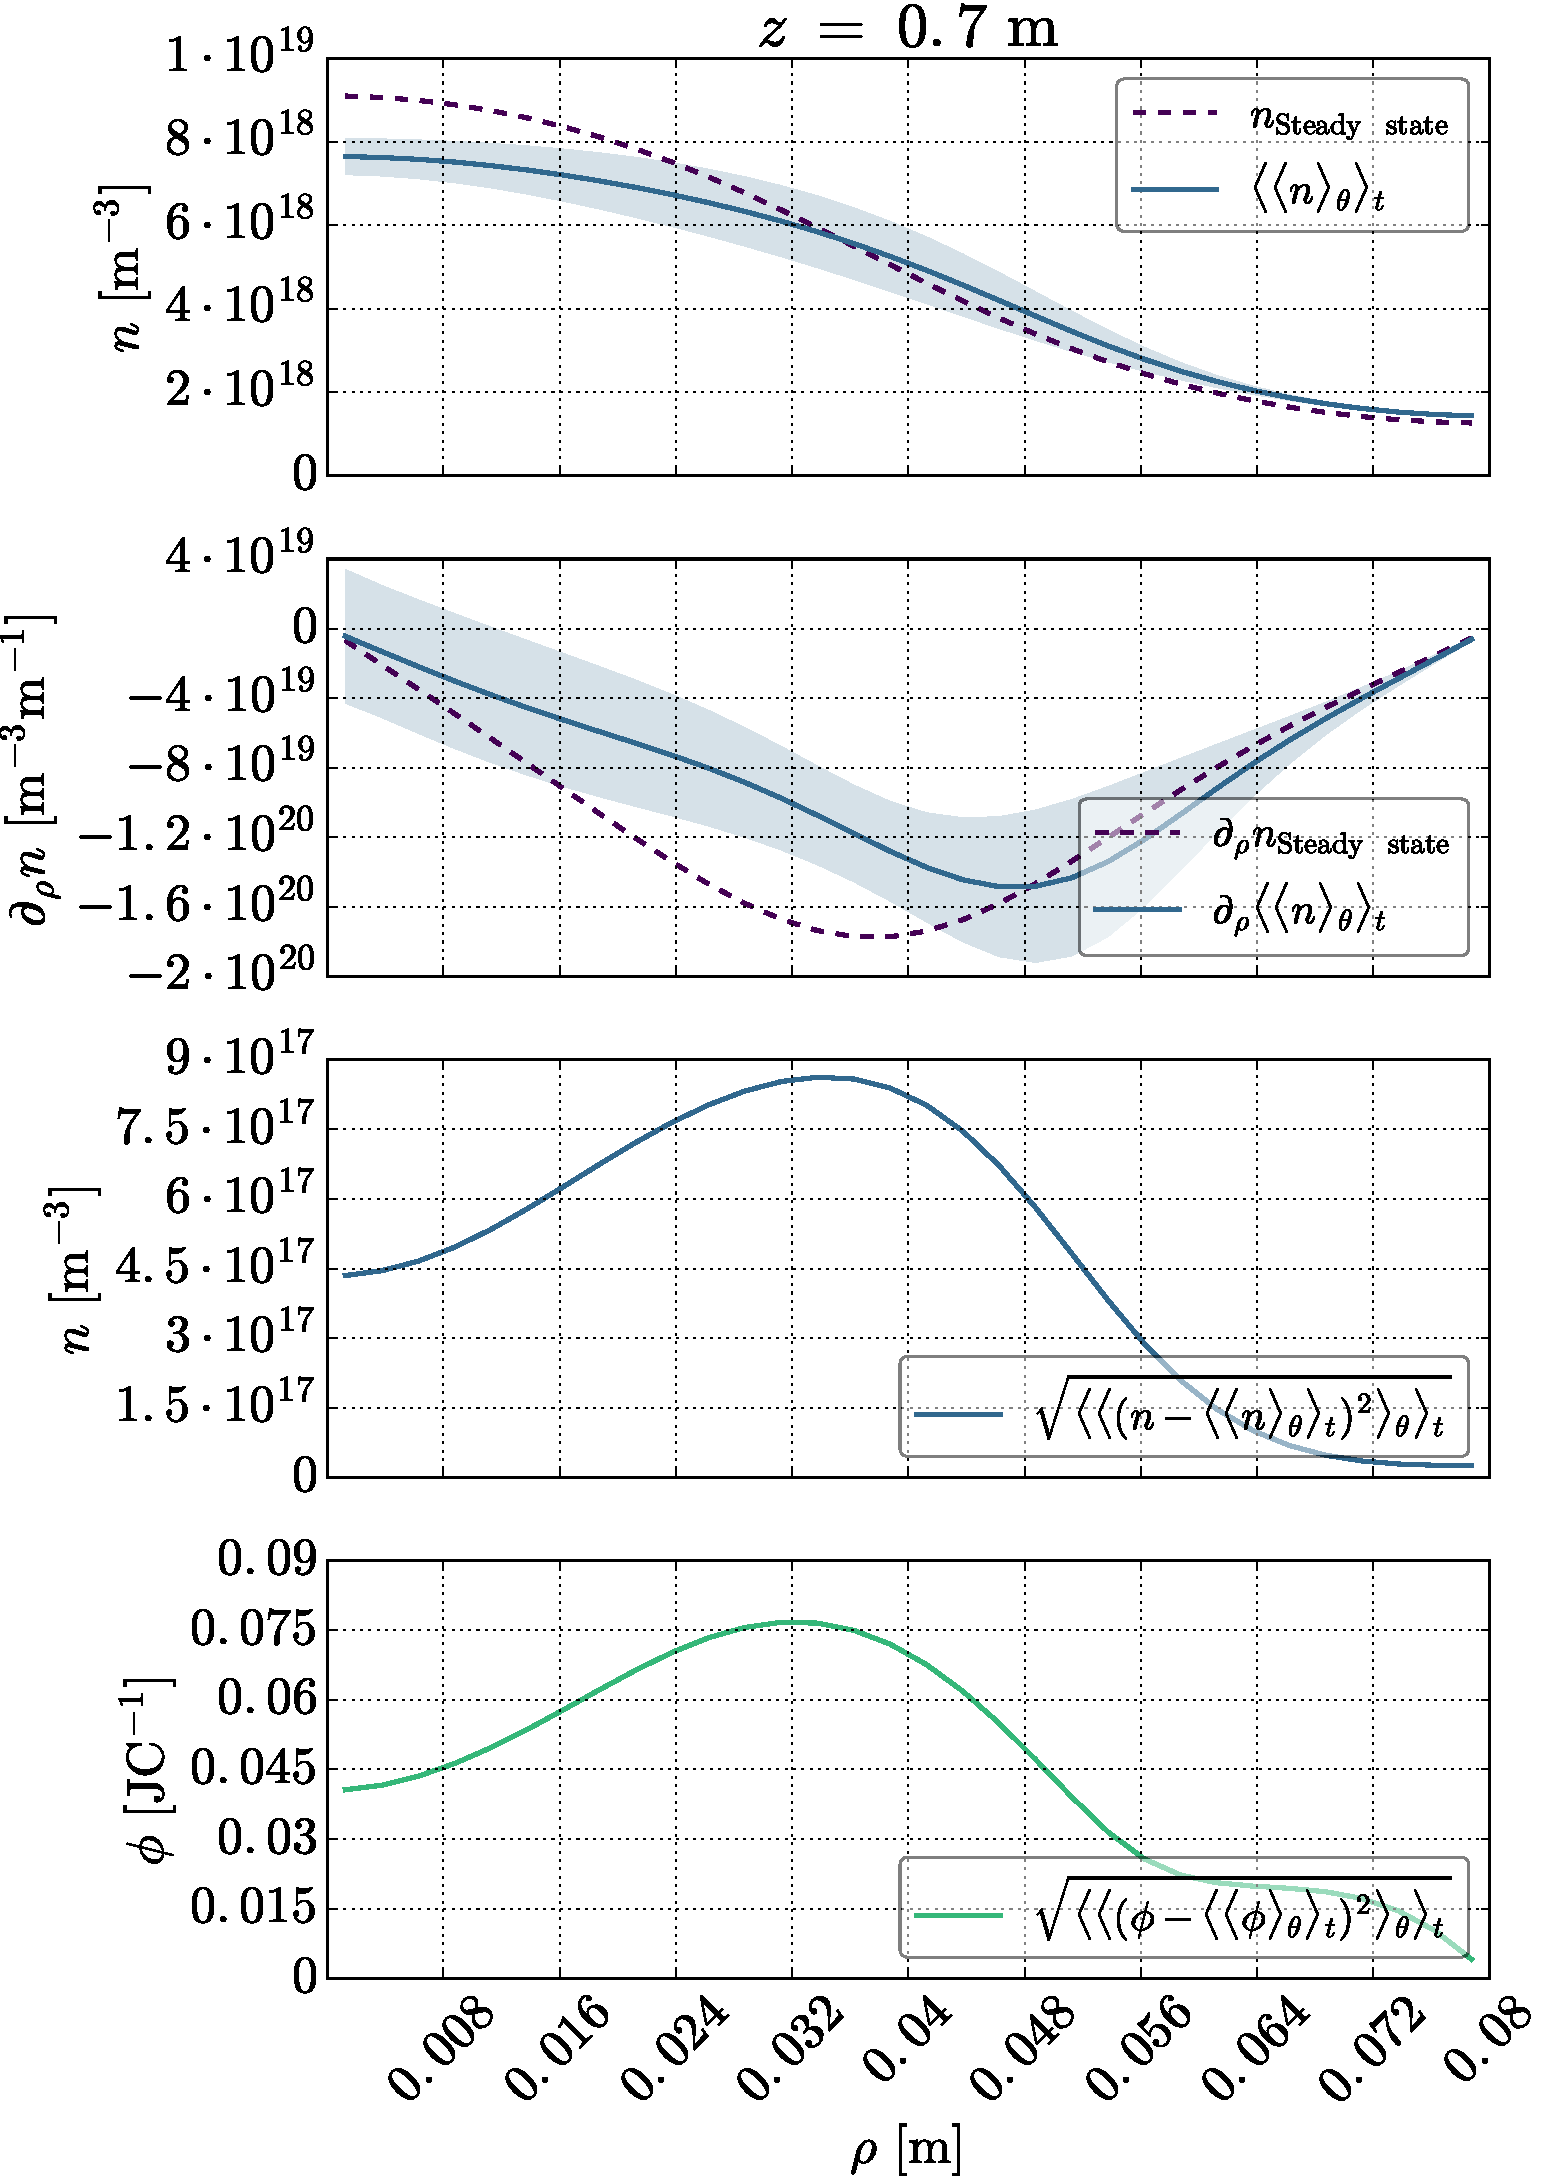
\includegraphics[width=1.0\textwidth]{fig/results/compareBouss/fluctProfiles008B}
    \caption{Steady state and averaged turbulent density profiles together with the radial distribution of the standard deviations of the fluctuations using the Boussinesq approximation with $B=0.08\T$.}
    \label{fig:posOfFluct008B}
\end{figure}
%
Finally, the skewness and kurtosis, shown in \cref{fig:skewKurt008B}, are investegated.
We observe that the system is platikurtic for all radii.
This reflects that the structure rotating around the center og the cylinder has a coherent character.
The skewness is no longer monotonically growing, but has a maximum close to the position of absolute largest gradient of the fluctuating profile.
%
\begin{figure}[htb]
    \centering
    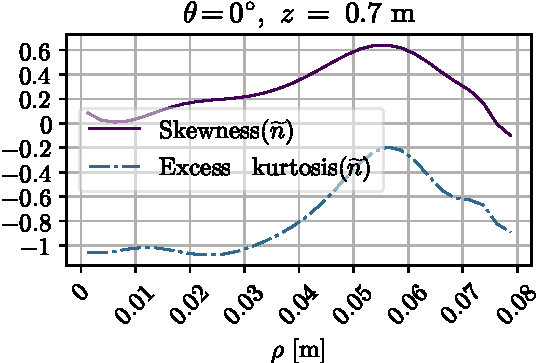
\includegraphics[width=1.0\textwidth]{fig/results/compareBouss/skewKurt008B}
    \caption{Skewness and kurtosis for $B=0.08\T$ using the Boussinesq approximation.}
    \label{fig:skewKurt008B}
\end{figure}
%
